\documentclass{article}
\usepackage{graphicx}
\usepackage[style=ieee]{biblatex} % Establecer el estilo de las referencias como IEEE
\usepackage{xcolor}
\usepackage{hyperref}
\usepackage{titletoc}
\usepackage{adjustbox}
\usepackage{amsmath}
\usepackage[spanish]{babel}

\usepackage{listings}
\hypersetup{
    colorlinks=true,
    linkcolor=blue, % Color del texto del enlace
    urlcolor=blue % Color del enlace
}

\usepackage{longtable} % Agrega el paquete longtable

\definecolor{mygreen}{RGB}{0,128,0}

\usepackage{array} % Para personalizar la tabla
\usepackage{booktabs} % Para líneas horizontales de mejor calidad
\usepackage{graphicx} % Paquete para incluir imágenes
\usepackage{float}

% Definir márgenes
\usepackage[margin=1in]{geometry}

\renewcommand{\contentsname}{\textcolor{mygreen}{Tabla de Contenidos}}

\begin{document}

\begin{titlepage}
    \centering
    % Logo de la Universidad
    
\includegraphics[width=0.48\textwidth]{logo_universidad.png}
    \par\vspace{2cm}

    % Nombre de la Universidad y detalles del curso
    {\Large \textbf{Universidad Nacional de Colombia} \par}
    \vspace{0.5cm}
    {\large Ingeniería de Sistemas y Computación \par}
    {\large 2025969 Modelos estocásticos y simulación en computación y comunicaciones (01)\par}
    \vspace{3cm}

    % Detalles del laboratorio y actividad
    {\large \textbf{Taller 2} \par}
    \vspace{3cm}

    % Lista de integrantes
    {\large \textbf{Integrantes:} \par}
    \vspace{0.5cm}
    \begin{tabular}{ll}
    Javier Andrés Tarazona Jiménez & jtarazonaj@unal.edu.co \\
    Yenifer Yulieth Mora Segura & ymoras@unal.edu.co \\
    Juan Esteban Carranza Salazar & jcarranza@unal.edu.co \\
    Grevy Joner Rincon Mejia & grrinconm@unal.edu.co \\
    Jefferson Duvan Ramirez Castañeda & jeramirezca@unal.edu.co \\
    Javier Andres Carrillo Carrasco & jacarrillo@unal.edu.co \\
    Diego Nicolas Ramirez Maldonado & dieramirezma@unal.edu.co \\
    \end{tabular}
    \par\vspace{3cm}

    % Fecha
    {\large Julio 21 de 2025 \par}
\end{titlepage}

\tableofcontents % Inserta la tabla de contenidos

\newpage % Salto de página para separar la tabla de contenidos del contenido del documento

% Contenido del artículo----------------------------------------------------------

%---------------------------------------------------------------------------------
% Intro --------------------------------------------------------------------------
%---------------------------------------------------------------------------------

\section{Introducción}\label{sec:intr}


%---------------------------------------------------------------------------------
% Marco Teórico ------------------------------------------------------------------
%---------------------------------------------------------------------------------

\section{Marco Teórico}\label{sec:marc}

\subsection{Modelos de Colas}
\subsubsection{Definición y Características}

Un \textbf{Sistema de Colas} es una estructura matemática utilizada para modelar situaciones en las que los "clientes" (que pueden ser personas, datos o tareas) llegan para ser atendidos por uno o más servidores. Este modelo es fundamental en áreas como telecomunicaciones, manufactura, logística, atención al cliente, y sistemas de información, ya que permite predecir y optimizar el rendimiento de sistemas que operan bajo condiciones de congestión o espera.

\begin{itemize}
    \item \textbf{Sistema de Colas:} Se define como un proceso estocástico en el que los clientes llegan a un punto de servicio y deben esperar hasta que el servicio esté disponible. Estos sistemas son caracterizados por tres componentes principales:
    \begin{itemize}
        \item \textbf{Llegadas:} El proceso que describe la llegada de clientes al sistema. Este proceso suele modelarse utilizando distribuciones de probabilidad, como la \textit{distribución de Poisson}, que describe el tiempo entre llegadas de manera aleatoria.
        \item \textbf{Cola:} El espacio de espera donde los clientes se sitúan hasta que se les ofrece servicio. La cola puede ser \textit{finita o infinita} dependiendo del modelo y de las restricciones del sistema.
        \item \textbf{Servicio:} El proceso mediante el cual el cliente es atendido por uno o más servidores. El tiempo de servicio es típicamente modelado utilizando distribuciones de probabilidad como la \textit{distribución exponencial}, la cual asume que el tiempo entre la finalización de un servicio y el inicio de otro es aleatorio y no sigue un patrón predecible.
    \end{itemize}
    
    \item \textbf{Características Clave de los Sistemas de Colas:} Los sistemas de colas se definen por varios factores que determinan su comportamiento y rendimiento. Las principales características de los sistemas de colas incluyen:
    \begin{itemize}
        \item \textbf{Tasa de Llegada (\(\lambda\)):} Es la frecuencia con la que los clientes llegan al sistema. Generalmente, se modela utilizando una \textit{distribución de Poisson} para representar llegadas independientes entre sí, lo que implica que el tiempo entre llegadas sigue una distribución \textit{exponencial}.
        \item \textbf{Tasa de Servicio (\(\mu\)):} Es la frecuencia con la que el servidor atiende a los clientes. Normalmente, el tiempo de servicio es representado por una distribución \textit{exponencial}.
        \item \textbf{Capacidad del Sistema:} La cantidad máxima de clientes que el sistema puede manejar en un momento dado. Algunos modelos de colas permiten una \textit{cola infinita}, mientras que otros pueden tener un número máximo de clientes que el sistema puede aceptar (por ejemplo, M/M/1 o M/M/c).
        \item \textbf{Número de Servidores (c):} En muchos sistemas de colas, un solo servidor puede atender a los clientes (como en el modelo M/M/1), pero en otros sistemas puede haber múltiples servidores trabajando simultáneamente en el servicio de diferentes clientes (por ejemplo, en el modelo M/M/c).
        \item \textbf{Disciplina de Servicio:} Define el orden en el que los clientes son atendidos dentro de la cola. Las más comunes incluyen \textit{FIFO} (First In, First Out), \textit{LIFO} (Last In, First Out), o \textit{SJF} (Shortest Job First). En la mayoría de los sistemas de colas, se asume que la disciplina es FIFO.
        \item \textbf{Tiempo de Espera:} Es el tiempo que un cliente pasa esperando en la cola antes de ser atendido. Es una de las métricas más importantes para evaluar la eficiencia de un sistema de colas, ya que refleja el nivel de congestión del sistema.
        \item \textbf{Utilización del Servidor (\(\rho\)):} Este parámetro describe el porcentaje de tiempo que un servidor está ocupado atendiendo a los clientes. Se calcula como la relación entre la tasa de llegada (\(\lambda\)) y la tasa de servicio (\(\mu\)):  
        \[
        \rho = \frac{\lambda}{\mu}
        \]
        Si \(\rho\) es cercano a 1, significa que el servidor está muy ocupado, lo que puede generar largos tiempos de espera y alta congestión.
    \end{itemize}

    \item \textbf{Importancia y Aplicaciones:} El estudio de los sistemas de colas es esencial para entender y optimizar el rendimiento de sistemas reales en los que se presentan tiempos de espera y congestión. Estos modelos no solo son útiles para analizar la eficiencia de sistemas de servicio, sino que también ayudan en la \textit{gestión de recursos} y la \textit{planificación operativa}. Ejemplos comunes de aplicaciones incluyen:
    \begin{itemize}
        \item \textbf{Telecomunicaciones:} En redes de computadoras y telecomunicaciones, los paquetes de datos pueden ser modelados como clientes en un sistema de colas, y los servidores como enrutadores o nodos de la red.
        \item \textbf{Manufactura:} En las líneas de producción, los productos que deben ser procesados en varias etapas son modelados como clientes que esperan en las estaciones de trabajo.
        \item \textbf{Servicios al Cliente:} En áreas como bancos, supermercados o servicios en línea, los clientes esperan ser atendidos, y el sistema de colas ayuda a optimizar la cantidad de personal necesario en diferentes momentos del día.
    \end{itemize}
\end{itemize}

\subsubsection{Clasificación de los Sistemas de Colas}
La clasificación de los sistemas de colas se basa en diversas características que determinan su estructura y comportamiento. Cada tipo de sistema tiene distintas implicaciones en su modelado matemático, así como en su aplicación práctica. Los sistemas de colas pueden clasificarse de acuerdo con varios factores, como el número de servidores, el comportamiento de las llegadas y los tiempos de servicio, y la capacidad del sistema.

A continuación, se presenta una clasificación de los sistemas de colas, basada en sus principales características estructurales y operativas.

\begin{itemize}
    \item \textbf{Según el Número de Servidores:}
    \begin{itemize}
        \item \textbf{M/M/1:} Este es el modelo más simple y comúnmente utilizado, donde 'M' representa una distribución de Poisson para las llegadas y una distribución exponencial para los tiempos de servicio. En este modelo, hay un único servidor (\(1\)), lo que significa que los clientes deben esperar para ser atendidos si el servidor está ocupado. Este modelo es ampliamente utilizado en situaciones con baja carga de tráfico o cuando solo está disponible un servidor para atender las solicitudes.
        \item \textbf{M/M/c:} En este caso, \(c\) representa el número de servidores. Este modelo es una extensión del M/M/1, y se utiliza cuando varios servidores están disponibles para atender a los clientes. Este tipo de sistema se usa comúnmente en centros de llamadas, hospitales o estaciones de servicio donde múltiples recursos están disponibles.
    \end{itemize}
    
    \item \textbf{Según la Distribución de las Llegadas:}
    \begin{itemize}
        \item \textbf{M/M/1:} En este caso, las llegadas siguen una distribución de Poisson, lo que implica que las llegadas son independientes y el tiempo entre llegadas sigue una distribución exponencial. Este modelo es adecuado para sistemas con llegadas aleatorias y sin patrones específicos.
        \item \textbf{G/G/1:} En este modelo, las llegadas y los tiempos de servicio siguen distribuciones generales, es decir, no están restringidos a distribuciones específicas como la Poisson o exponencial. Este modelo es más flexible y se utiliza cuando las llegadas o los tiempos de servicio no siguen una distribución simple y se requiere un modelado más general.
    \end{itemize}
    
    \item \textbf{Según la Disciplina de Servicio:}
    \begin{itemize}
        \item \textbf{FIFO (First In, First Out):} Esta es la disciplina de servicio más común y se asume en la mayoría de los modelos de colas. Los clientes son atendidos en el orden en que llegan al sistema, es decir, el primero en llegar es el primero en ser atendido.
        \item \textbf{LIFO (Last In, First Out):} En esta disciplina, el último cliente en llegar es el primero en ser atendido. Este modelo es menos común, pero puede aplicarse en situaciones donde la atención urgente a los clientes más recientes es prioritaria, como en ciertos sistemas de caché de computadoras.
        \item \textbf{SJF (Shortest Job First):} En este modelo, los clientes que requieren el servicio más corto son atendidos primero. Esta disciplina se utiliza principalmente en entornos donde los recursos deben asignarse de manera eficiente, como en el procesamiento de tareas informáticas.
    \end{itemize}
    
    \item \textbf{Según la Capacidad del Sistema:}
    \begin{itemize}
        \item \textbf{Sistema de Cola Infinita:} En este tipo de sistema, la capacidad de la cola no está limitada. Esto significa que no hay restricciones sobre cuántos clientes pueden esperar en la cola. Este modelo es adecuado para sistemas de colas con una alta demanda y sin límites físicos, como ciertos sistemas informáticos o redes de telecomunicaciones.
        \item \textbf{Sistema de Cola Finita:} En contraste, en un sistema de cola finita, existe un límite máximo en el número de clientes que pueden estar esperando en la cola en un momento dado. Los clientes adicionales que lleguen cuando la cola esté llena serán rechazados o perderán el servicio. Este tipo de sistema es más adecuado para entornos donde los recursos son limitados, como en estaciones de servicio o ciertos tipos de servicios al cliente.
    \end{itemize}
\end{itemize}

\subsubsection{Aplicaciones de los Modelos de Colas}

Los modelos de colas son fundamentales en diversas disciplinas como ingeniería, informática y telecomunicaciones, así como en otros sectores donde la eficiencia del servicio es crucial. La teoría de colas se aplica en situaciones que involucran congestión, asignación de recursos limitados y tiempos de espera. Su utilización adecuada puede generar mejoras sustanciales en la gestión de recursos y la optimización de procesos.

A continuación, se describen algunas de las aplicaciones más relevantes de los modelos de colas en distintos campos:

\begin{itemize}
    \item \textbf{Telecomunicaciones:}
    En las redes de telecomunicaciones, los sistemas de colas son fundamentales para modelar el comportamiento de las transmisiones de datos. Los paquetes de datos, que actúan como "clientes", llegan a un servidor de red (como un enrutador o un conmutador) y esperan para ser procesados o transmitidos. Los modelos de colas permiten evaluar la congestión en las redes y diseñar algoritmos para asignar recursos de manera eficiente, minimizando el tiempo de espera y la probabilidad de pérdida de paquetes. En particular, el modelo \textit{M/M/1} es ampliamente utilizado para estudiar redes con un solo servidor, mientras que modelos más complejos como \textit{M/M/c} son utilizados para estudiar redes con múltiples servidores.
    
    Los sistemas de colas también se utilizan en el análisis de la capacidad de redes celulares y de Internet, optimizando la asignación de recursos en momentos de alta demanda. El tráfico de datos en las redes de telecomunicaciones puede ser modelado como un proceso de llegada estocástico, y el rendimiento de la red puede ser analizado en términos de la tasa de pérdida de paquetes, el tiempo de espera y la utilización de los recursos.

    \item \textbf{Sistemas de Computación y Redes:}
    En los sistemas informáticos, los modelos de colas se emplean para analizar la gestión de tareas en servidores, sistemas de bases de datos y procesadores. La ejecución de tareas en un servidor puede ser vista como un sistema de colas, donde los procesos llegan para ser ejecutados y deben esperar su turno en la cola. Estos modelos son esenciales en la planificación de cargas de trabajo, la asignación de recursos y la gestión de sistemas multitarea.

    En las redes de computadoras, los paquetes de datos que esperan ser transmitidos a través de los nodos de la red se tratan como clientes en un sistema de colas. La optimización de redes de computadoras implica minimizar la congestión y los retrasos en las transmisiones, lo que se puede lograr mediante el ajuste adecuado de los recursos disponibles, el enrutamiento de paquetes y la gestión de la calidad del servicio (QoS). Los modelos de colas también son cruciales para la gestión de centros de datos y servidores de bases de datos, donde múltiples procesos compiten por el acceso a recursos limitados.

    \item \textbf{Manufactura y Producción:}
    En el ámbito de la manufactura, los modelos de colas son utilizados para estudiar las líneas de producción, en las que los productos o materiales deben pasar a través de diferentes estaciones de trabajo. Los productos que esperan ser procesados son modelados como clientes, y las estaciones de trabajo actúan como servidores que brindan el servicio requerido. Estos modelos permiten evaluar la eficiencia de las líneas de producción, identificando posibles cuellos de botella y optimizando el flujo de materiales.

    Los sistemas de colas también se utilizan en la planificación de la capacidad de los sistemas de producción, ayudando a decidir el número óptimo de estaciones de trabajo, el número de operarios y el diseño de la línea de producción para minimizar los tiempos de espera y mejorar la eficiencia operativa. En un entorno de producción, los clientes pueden representar productos que deben ser ensamblados, y los servidores son las máquinas o estaciones de trabajo que realizan las tareas correspondientes.

    \item \textbf{Servicios Bancarios y Financieros:}
    Los sistemas de colas son ampliamente aplicados en la gestión de servicios bancarios y financieros, donde los clientes esperan ser atendidos por cajeros o asesores. En este caso, el objetivo es minimizar los tiempos de espera para los clientes y, al mismo tiempo, garantizar una utilización eficiente de los recursos disponibles, como cajeros y asesores. Los modelos de colas pueden ayudar a determinar el número adecuado de cajeros o personal de atención en diferentes momentos del día, basándose en la tasa de llegada de clientes y el tiempo promedio de servicio.

    Los sistemas de colas también se utilizan en el análisis de los servicios automatizados, como los cajeros automáticos (ATM), donde los clientes realizan transacciones sin la necesidad de interacción humana. En estos sistemas, los modelos de colas permiten optimizar la ubicación de los cajeros, la cantidad de terminales disponibles y la gestión de las demandas fluctuantes en función de la hora del día.

    \item \textbf{Atención al Cliente y Centros de Llamadas:}
    En el ámbito de la atención al cliente, los modelos de colas son esenciales para gestionar centros de llamadas y otros servicios donde los clientes deben esperar ser atendidos. Los centros de llamadas, donde los clientes llaman para obtener soporte o información, pueden modelarse como sistemas de colas, con las llamadas representando a los clientes y los operadores como los servidores. La optimización de estos sistemas involucra determinar la cantidad adecuada de operadores para minimizar los tiempos de espera y mejorar la calidad del servicio al cliente.

    Los modelos de colas también se utilizan en el análisis de la eficiencia de los sistemas automáticos de atención al cliente, como los sistemas IVR (respuesta de voz interactiva), que permiten que los clientes interactúen con un sistema automatizado antes de ser atendidos por un operador. En estos casos, los modelos de colas pueden ayudar a evaluar el impacto de la automatización en los tiempos de espera y en la satisfacción del cliente.

    \item \textbf{Transporte Público:}
    En el transporte público, los sistemas de colas se utilizan para modelar el flujo de pasajeros en estaciones de trenes, aeropuertos y paradas de autobuses. Los modelos permiten estudiar la distribución de los pasajeros en diferentes rutas y determinar el número óptimo de vehículos necesarios en cada momento para satisfacer la demanda de manera eficiente. Los modelos de colas también se aplican para gestionar la congestión en las horas punta y reducir los tiempos de espera de los pasajeros.

    Además, estos modelos pueden ser útiles en el análisis de la asignación de recursos, como la cantidad de vehículos, la frecuencia de los viajes y la distribución de los pasajeros en las diferentes rutas del sistema de transporte. La optimización de estos aspectos ayuda a mejorar la eficiencia operativa y la satisfacción de los usuarios.

    \item \textbf{Salud y Hospitales:}
    En el sector salud, los modelos de colas se aplican para estudiar el flujo de pacientes a través de diferentes etapas de atención, como consultas médicas, diagnósticos y procedimientos. Estos modelos permiten analizar la eficiencia de los recursos, como médicos, enfermeras y equipos de diagnóstico, y optimizar la programación de citas para reducir los tiempos de espera y mejorar la calidad del servicio. Además, los modelos de colas se utilizan para gestionar la capacidad de los hospitales y las unidades de emergencia, donde el número de pacientes puede superar rápidamente la capacidad del sistema de salud.

    \item \textbf{Sistemas de Distribución y Logística:}
    En la logística y distribución, los modelos de colas se utilizan para modelar los centros de distribución, almacenes y líneas de ensamblaje. Los productos o materiales en espera de ser procesados o distribuidos son tratados como clientes en un sistema de colas. Los modelos permiten optimizar la operación de estos sistemas, minimizando los tiempos de espera y maximizando la eficiencia operativa.

    Además, los modelos de colas se utilizan en la simulación de sistemas de gestión de inventarios y distribución de recursos, ayudando a mejorar la planificación de la cadena de suministro, la asignación de recursos y la programación de las entregas.

\end{itemize}

\subsection{Modelo M/M/1}
\subsubsection{Descripción Técnica del Modelo}

El modelo M/M/1 es uno de los modelos más simples y fundamentales en la teoría de colas, utilizado para describir sistemas en los que los clientes llegan de manera aleatoria y deben esperar para ser atendidos por un solo servidor. La notación \textit{M/M/1} se desglosa de la siguiente manera:

\begin{itemize}
    \item \textbf{M} (Markoviano) para las llegadas: El proceso de llegadas de clientes sigue una \textit{distribución de Poisson}, lo que implica que las llegadas son aleatorias y ocurren a una tasa constante, con interludios entre llegadas que siguen una \textit{distribución exponencial}.
    
    \item \textbf{M} (Markoviano) para el servicio: El tiempo de servicio sigue una \textit{distribución exponencial}, lo que implica que la tasa de servicio es constante y cada cliente es atendido de forma independiente de los anteriores.
    
    \item \textbf{1}: Indica que el sistema cuenta con \textbf{un solo servidor} que atiende a los clientes que llegan.
\end{itemize}

Este modelo se basa en suponer que tanto las llegadas como los tiempos de servicio son procesos estocásticos, y como tal, la teoría de colas aplicada al modelo M/M/1 está fuertemente influenciada por la teoría de procesos de Markov.

\begin{itemize}
    \item \textbf{Flujo del Modelo M/M/1:} En este modelo, los clientes llegan a la cola según un proceso de Poisson, y los tiempos de servicio se distribuyen de forma exponencial. Cuando un cliente llega y el servidor está ocupado, el cliente debe esperar en la cola hasta que el servidor se encuentre disponible. Si el servidor está libre en el momento de la llegada, el cliente es atendido inmediatamente.
    
    \item \textbf{Funcionamiento:} El sistema opera bajo un conjunto de reglas que permiten la modelización de los siguientes aspectos:
    \begin{itemize}
        \item \textit{Llegadas:} Las llegadas de clientes son completamente aleatorias, con una tasa de llegada promedio de \( \lambda \) clientes por unidad de tiempo. La llegada de clientes es independiente de las llegadas anteriores, lo que implica que las llegadas siguen un proceso de \textit{Poisson}.
        
        \item \textit{Servicio:} El servidor atiende a los clientes según una tasa de servicio \( \mu \), también constante. Los tiempos de servicio son independientes entre sí y siguen una distribución \textit{exponencial}, lo que significa que el tiempo de servicio entre cada cliente es aleatorio, pero con una tasa promedio de \( \mu \).
    \end{itemize}
    
    \item \textbf{Representación Matemática:} La tasa de utilización del servidor \( \rho \) es un parámetro clave del modelo M/M/1 y se define como la relación entre la tasa de llegada \( \lambda \) y la tasa de servicio \( \mu \):
    \[
    \rho = \frac{\lambda}{\mu}
    \]
    Donde \( \rho \) debe ser menor que 1 para que el sistema sea estable. Si \( \rho \) es mayor o igual a 1, el sistema no es estable y los tiempos de espera pueden crecer indefinidamente.
    
    \item \textbf{Importancia del Modelo M/M/1:} El modelo M/M/1 se utiliza como base para el análisis de otros sistemas de colas más complejos. Su simplicidad y facilidad de análisis matemático lo hacen ideal para modelar y estudiar el comportamiento de sistemas básicos de espera. A pesar de su simplicidad, proporciona una visión clara de cómo el comportamiento de los sistemas de colas depende de las tasas de llegada y servicio, y cómo estos factores afectan las métricas clave como los tiempos de espera y la utilización del servidor.
    
    Este modelo sirve como una aproximación útil en muchos escenarios prácticos donde el servicio es aleatorio y el sistema se puede simplificar a un solo servidor, permitiendo realizar estimaciones y predicciones sobre el rendimiento de sistemas reales.
\end{itemize}

\subsubsection{Supuestos y Restricciones}

El modelo M/M/1, aunque es uno de los más sencillos y utilizados en la teoría de colas, se basa en una serie de supuestos que deben cumplirse para que los resultados del modelo sean válidos. Estos supuestos permiten la simplificación matemática del modelo, pero también presentan limitaciones en su aplicabilidad en escenarios del mundo real. A continuación, se describen los supuestos fundamentales y las restricciones asociadas al modelo M/M/1:

\begin{itemize}
    \item \textbf{Llegadas de Clientes Según una Distribución de Poisson:} 
    El modelo M/M/1 asume que las llegadas de clientes siguen una \textit{distribución de Poisson}. Esto implica que las llegadas son completamente aleatorias y ocurren a una tasa constante \( \lambda \), con intervalos de tiempo entre llegadas que siguen una \textit{distribución exponencial}. En la práctica, esto puede ser una simplificación excesiva en muchos sistemas, ya que en algunos contextos las llegadas pueden seguir distribuciones más complejas.
    
    \item \textbf{Tiempo de Servicio Exponencial:} 
    El tiempo que cada cliente pasa siendo atendido sigue una \textit{distribución exponencial} con tasa \( \mu \). Esto implica que el tiempo de servicio es aleatorio y tiene una media constante. En muchos casos prácticos, los tiempos de servicio pueden no ser exponenciales y pueden variar dependiendo del tipo de tarea, lo que limita la aplicabilidad directa del modelo.
    
    \item \textbf{Un Solo Servidor:} 
    El modelo M/M/1 se limita a un sistema con \textbf{un solo servidor} (\(1\)). Este supuesto implica que solo hay un punto de servicio para todos los clientes que llegan, lo cual es una simplificación en sistemas más complejos que cuentan con múltiples servidores. Los sistemas con varios servidores requieren la extensión del modelo M/M/1, como el modelo M/M/c.
    
    \item \textbf{Disciplina de Servicio FIFO:} 
    Se asume que los clientes son atendidos siguiendo la disciplina \textit{FIFO} (First In, First Out), lo que significa que el cliente que llega primero será el primero en ser atendido. En la práctica, sin embargo, existen otras disciplinas de servicio, como \textit{LIFO} (Last In, First Out) o \textit{SJF} (Shortest Job First), que pueden no cumplir con esta suposición y pueden alterar significativamente el comportamiento del sistema.
    
    \item \textbf{Capacidad del Sistema Infinita:} 
    El modelo M/M/1 asume que la cola puede almacenar un número ilimitado de clientes. Esto significa que no hay restricción en el número de clientes que pueden esperar para ser atendidos. En sistemas reales, la capacidad de las colas suele ser limitada, lo que puede llevar a la pérdida de clientes cuando el sistema está lleno, lo que no está reflejado en el modelo M/M/1.
    
    \item \textbf{Estabilidad del Sistema (\( \rho < 1 \)):} 
    Para que el sistema M/M/1 sea estable, se requiere que la tasa de llegada \( \lambda \) sea menor que la tasa de servicio \( \mu \), es decir, que \( \rho = \frac{\lambda}{\mu} < 1 \). Este supuesto implica que el servidor es lo suficientemente rápido como para atender a todos los clientes que llegan al sistema sin que la cola crezca de manera indefinida. Si \( \rho \geq 1 \), el sistema será inestable y los tiempos de espera crecerán sin límite, lo que es una restricción importante a tener en cuenta en la práctica.
\end{itemize}

 \textbf{Restricciones y Limitaciones del Modelo:}
El modelo M/M/1 es extremadamente útil para análisis básicos y sirve como una aproximación adecuada en muchas situaciones. Sin embargo, las suposiciones de llegadas de Poisson, tiempos de servicio exponenciales, un solo servidor y cola infinita son simplificaciones que no siempre se ajustan a la realidad. En escenarios más complejos, como sistemas con múltiples servidores, tiempos de servicio no exponenciales o llegadas que no siguen una distribución de Poisson, es necesario considerar modelos más avanzados o utilizar la simulación de colas.

A pesar de sus limitaciones, el modelo M/M/1 sigue siendo una herramienta valiosa para comprender los principios fundamentales de la teoría de colas y sirve como base para la construcción de modelos más complejos y realistas.

\subsubsection{Propiedades Clave}

El modelo M/M/1, a pesar de su simplicidad, presenta varias propiedades fundamentales que permiten analizar su comportamiento y rendimiento. Estas propiedades son esenciales para comprender cómo las tasas de llegada y servicio afectan las métricas clave del sistema, como los tiempos de espera y la utilización del servidor. A continuación, se detallan las propiedades más importantes de este modelo:

\begin{itemize}
    \item \textbf{Utilización del Servidor (\(\rho\)):} 
    La tasa de utilización del servidor, denotada por \( \rho \), es una medida crucial del modelo M/M/1. Se define como la relación entre la tasa de llegada \( \lambda \) y la tasa de servicio \( \mu \):

    \[
    \rho = \frac{\lambda}{\mu}
    \]

    Esta propiedad indica la fracción del tiempo que el servidor está ocupado. Para que el sistema sea estable, \( \rho \) debe ser menor que 1. Si \( \rho \) es igual o superior a 1, el sistema no es estable, lo que puede llevar a tiempos de espera infinitos. En la práctica, \( \rho \) proporciona una indicación del nivel de carga del sistema: valores cercanos a 1 indican que el sistema está cerca de su capacidad máxima.

    \item \textbf{Tiempo Promedio de Espera en la Cola (\( W_q \)):} 
    El tiempo promedio que un cliente pasa esperando en la cola antes de ser atendido es una métrica crítica en los sistemas de colas. En el modelo M/M/1, el tiempo de espera en la cola está dado por la siguiente fórmula:

    \[
    W_q = \frac{\lambda}{\mu (\mu - \lambda)}
    \]

    Este tiempo es inversamente proporcional a la diferencia entre la tasa de servicio \( \mu \) y la tasa de llegada \( \lambda \). A medida que la tasa de llegada aumenta, el tiempo de espera en la cola también aumenta, lo que subraya la importancia de mantener un balance adecuado entre estas dos tasas para evitar largas colas.

    \item \textbf{Tiempo Promedio de Espera en el Sistema (\( W \)):} 
    El tiempo total que un cliente pasa en el sistema, desde su llegada hasta que termina su servicio, es la suma del tiempo de espera en la cola y el tiempo de servicio. En el modelo M/M/1, el tiempo promedio de espera en el sistema se calcula mediante la siguiente fórmula:

    \[
    W = W_q + \frac{1}{\mu}
    \]

    Dado que el tiempo de servicio es inversamente proporcional a \( \mu \), un mayor valor de \( \mu \) (es decir, un servidor más rápido) resulta en un menor tiempo de espera total en el sistema.

    \item \textbf{Número Promedio de Clientes en la Cola (\( L_q \)):} 
    El número promedio de clientes que se encuentran en la cola en un momento dado es una propiedad fundamental en el análisis de sistemas de colas. En el modelo M/M/1, este número se calcula como:

    \[
    L_q = \lambda^2 / (\mu (\mu - \lambda))
    \]

    Este valor refleja la acumulación de clientes en espera y es mayor cuando \( \lambda \) se acerca a \( \mu \), lo que indica que el sistema está cerca de su capacidad máxima.

    \item \textbf{Número Promedio de Clientes en el Sistema (\( L \)):} 
    El número total de clientes en el sistema (que incluye tanto los clientes en la cola como aquellos siendo atendidos) se calcula sumando el número promedio de clientes en la cola \( L_q \) y la tasa de servicio \( \lambda / \mu \), es decir, el número promedio de clientes siendo atendidos:

    \[
    L = L_q + \frac{\lambda}{\mu}
    \]

    Esta propiedad proporciona una medida global de la cantidad de clientes que están siendo atendidos y esperando en el sistema. Al igual que con los tiempos de espera, el número de clientes en el sistema aumenta a medida que \( \lambda \) se aproxima a \( \mu \).

    \item \textbf{Probabilidad de que el Sistema esté Vacío (\( P_0 \)):} 
    La probabilidad de que no haya ningún cliente en el sistema en un momento dado, es decir, la probabilidad de que el sistema esté vacío, está dada por:

    \[
    P_0 = 1 - \rho
    \]

    Este valor es importante porque representa la probabilidad de que el servidor no esté ocupado, lo cual es relevante para la gestión de recursos y la evaluación de la eficiencia operativa.

    \item \textbf{Distribución de Probabilidad de Clientes en el Sistema:}
    La probabilidad de que haya \( n \) clientes en el sistema en un momento dado, denotada como \( P_n \), se puede calcular mediante la fórmula:

    \[
    P_n = (1 - \rho) \rho^n
    \]

    Esta fórmula describe cómo varía la probabilidad de que el sistema contenga un número determinado de clientes. La distribución muestra que a medida que \( n \) aumenta, la probabilidad de tener muchos clientes en el sistema disminuye exponencialmente, lo que indica que el modelo M/M/1 tiende a tener menos clientes a medida que la carga de tráfico disminuye.

\end{itemize}

\subsection{Teoría Matemática de las Colas}
\subsubsection{Teoría Probabilística Aplicada}
La modelación de sistemas de colas recurre a herramientas de probabilidad y procesos estocásticos que permitan describir la evolución del número de clientes en el sistema. A continuación se presentan los conceptos y resultados más generales:

\begin{itemize}
    \item \textbf{Proceso de Poisson y tiempos exponenciales:}  
    Un proceso de llegadas se modela frecuentemente como un \textit{proceso de Poisson} de tasa \(\lambda\), de modo que los intervalos entre llegadas son variables aleatorias \(\{T_i\}\) independientes con distribución exponencial
    \[
      \Pr\{T_i > t\} = e^{-\lambda t}.
    \]
    De forma análoga, si los tiempos de servicio son exponenciales de parámetro \(\mu\), se aprovecha la propiedad \textit{memoryless}
    \(\Pr\{T>s+t\mid T>s\}=\Pr\{T>t\}\).
    
    \item \textbf{Procesos de nacimiento–muerte:}  
    El número de clientes \(X(t)\) en un sistema de colas puede describirse por un proceso de nacimiento y muerte con tasas de nacimiento \(\{\lambda_n\}\) y de muerte \(\{\mu_n\}\). La matriz generadora \(Q=[q_{ij}]\) viene dada por
    \[
      q_{n,n+1}=\lambda_n,\quad
      q_{n,n-1}=\mu_n,\quad
      q_{n,n}=-(\lambda_n+\mu_n).
    \]
    
    \item \textbf{Ecuaciones de Kolmogorov (forward):}  
    Las probabilidades transitorias \(P_n(t)=\Pr\{X(t)=n\}\) satisfacen
    \[
      \frac{d}{dt}P_n(t)
        = \lambda_{n-1}P_{n-1}(t)
        + \mu_{n+1}P_{n+1}(t)
        - (\lambda_n+\mu_n)P_n(t),
    \]
    con condiciones de frontera adecuadas y \(\sum_nP_n(t)=1\).
    
    \item \textbf{Distribución estacionaria:}  
    En régimen estacionario (\(dP_n/dt=0\)) las \textit{ecuaciones de balance}  
    \(\lambda_{n-1}\pi_{n-1} + \mu_{n+1}\pi_{n+1} = (\lambda_n+\mu_n)\pi_n\)  
    se complementan con la normalización \(\sum_n\pi_n=1\). Para procesos birth–death se obtiene
    \[
      \pi_n = \pi_0 \prod_{i=0}^{n-1}\frac{\lambda_i}{\mu_{i+1}}.
    \]
    
    \item \textbf{PASTA (Poisson Arrivals See Time Averages):}  
    Cuando las llegadas siguen Poisson, la fracción de llegadas que encuentran el sistema en estado \(n\) coincide con la probabilidad estacionaria \(\pi_n\). Esto confirma la validez de comparar medidas de simulación (por llegada) con valores teóricos.
    
    \item \textbf{Ley de Little:}  
    De manera completamente general, en cualquier sistema estable se cumple
    \[
      L = \lambda \, W,
    \]
    donde \(L\) es el número promedio de clientes en el sistema, \(\lambda\) la tasa efectiva de llegadas, y \(W\) el tiempo promedio que un cliente pasa en el sistema.
\end{itemize}


\subsubsection{Cálculos de Probabilidades en Sistemas de Colas}
El cálculo de probabilidades en sistemas de colas es fundamental para entender el comportamiento de los sistemas y predecir su rendimiento en diferentes condiciones. A continuación, se presentan los principales métodos para calcular probabilidades clave que describen el estado del sistema, como el número de clientes en la cola y el tiempo de espera.

\begin{itemize}
    \item \textbf{Distribución Estacionaria:}  
    En los sistemas de colas en régimen estacionario, las probabilidades de encontrar el sistema en un estado específico (\(n\) clientes en el sistema) son fundamentales para la caracterización del sistema. Para los sistemas de colas clásicos como el modelo M/M/1, la distribución estacionaria \(P_n\) de encontrar \(n\) clientes en el sistema está dada por la fórmula
    \[
      P_n = (1 - \rho)\,\rho^n, \quad \text{para} \quad n = 0, 1, 2, \dots,
    \]
    donde \( \rho = \frac{\lambda}{\mu} \) es la tasa de utilización del servidor. Este modelo describe cómo la probabilidad de que el sistema contenga \(n\) clientes decae exponencialmente a medida que aumenta \(n\), con una probabilidad máxima de que el sistema esté vacío (\(P_0\)).

    \item \textbf{Probabilidad de que el sistema esté vacío (\(P_0\)):}  
    En cualquier sistema de colas M/M/1, la probabilidad de que no haya clientes en el sistema, es decir, que el sistema esté vacío, es una métrica clave para la evaluación del rendimiento del sistema. Para el modelo M/M/1, esta probabilidad se calcula como:
    \[
      P_0 = 1 - \rho = 1 - \frac{\lambda}{\mu}.
    \]
    Si el sistema está vacío, significa que el servidor está disponible para atender a un nuevo cliente.

    \item \textbf{Número Promedio de Clientes en el Sistema (\(L\)):}  
    El número promedio de clientes en el sistema, que incluye tanto a los clientes en la cola como los que están siendo atendidos, se calcula utilizando la probabilidad estacionaria y la distribución de Poisson. Para el modelo M/M/1, el número promedio de clientes en el sistema \(L\) es dado por:
    \[
      L = \sum_{n=0}^{\infty} n\,P_n = \frac{\rho}{1 - \rho}.
    \]
    Esta fórmula indica que el número promedio de clientes en el sistema aumenta con la tasa de llegada \(\lambda\) y disminuye con la tasa de servicio \(\mu\). A medida que la tasa de llegada se aproxima a la tasa de servicio (\(\rho \to 1\)), el número promedio de clientes en el sistema crece sin límites.

    \item \textbf{Tiempo Promedio de Espera en el Sistema (\(W\)):}  
    El tiempo promedio que un cliente pasa en el sistema, desde que llega hasta que es atendido, está relacionado con el número promedio de clientes en el sistema a través de la conocida \textit{ley de Little}, que establece que:
    \[
      W = \frac{L}{\lambda}.
    \]
    Esto implica que el tiempo promedio de espera aumenta conforme se incrementa el número de clientes en el sistema, lo que a su vez depende de la tasa de llegada y la tasa de servicio.

    \item \textbf{Tiempo Promedio de Espera en la Cola (\(W_q\)):}  
    El tiempo promedio que un cliente pasa esperando en la cola antes de ser atendido es una métrica clave para evaluar la eficiencia de un sistema de colas. En el modelo M/M/1, el tiempo de espera en la cola \(W_q\) se puede calcular con la siguiente fórmula:
    \[
      W_q = \frac{\lambda}{\mu(\mu - \lambda)}.
    \]
    Este tiempo es inversamente proporcional a la diferencia entre la tasa de servicio \( \mu \) y la tasa de llegada \( \lambda \). A medida que la tasa de llegada aumenta, el tiempo de espera en la cola se incrementa, lo que subraya la importancia de gestionar adecuadamente la tasa de servicio.

    \item \textbf{Número Promedio de Clientes en la Cola (\(L_q\)):}  
    El número promedio de clientes que esperan en la cola, antes de ser atendidos, se obtiene mediante la fórmula:
    \[
      L_q = \lambda^2 / (\mu(\mu - \lambda)).
    \]
    Similar al tiempo de espera, el número de clientes en la cola aumenta con la tasa de llegada y disminuye con la tasa de servicio. Cuando la tasa de llegada \( \lambda \) se aproxima a la tasa de servicio \( \mu \), el número de clientes en la cola crece significativamente.

    \item \textbf{Probabilidad de Pérdida de Clientes:}  
    En sistemas con capacidad finita o que utilizan técnicas de abandono, la probabilidad de que un cliente sea rechazado o pierda el servicio debido a la falta de espacio en la cola o los servidores es un cálculo importante. En sistemas de colas con pérdida, esta probabilidad depende de la capacidad del sistema y de las tasas de llegada y servicio.
\end{itemize}


\subsection{Simulación de Sistemas de Colas}
\subsubsection{Técnicas de Simulación}
La simulación de sistemas de colas es una herramienta fundamental cuando los métodos analíticos no son viables o cuando se desea obtener una estimación más precisa del comportamiento de un sistema en situaciones complejas. Existen diversas técnicas de simulación utilizadas para modelar y analizar los sistemas de colas, cada una con sus características y aplicaciones específicas.

En esta subsección se describen las principales técnicas utilizadas en la simulación de sistemas de colas:

\begin{itemize}
    \item \textbf{Simulación de Monte Carlo:}  
    La \textit{simulación de Monte Carlo} es un enfoque basado en la generación de números aleatorios para modelar y analizar sistemas estocásticos. Esta técnica se utiliza para obtener estimaciones de variables de interés mediante la repetición de simulaciones del sistema bajo diferentes condiciones. En el contexto de las colas, se generan secuencias de llegadas y tiempos de servicio, y se simula el comportamiento del sistema en función de estos parámetros. La principal ventaja de esta técnica es su capacidad para manejar sistemas con configuraciones complejas, donde las fórmulas analíticas no están disponibles o son difíciles de aplicar.

    En un sistema de colas M/M/1, por ejemplo, se generan números aleatorios para simular los tiempos entre llegadas (según una distribución exponencial con parámetro \( \lambda \)) y los tiempos de servicio (según una distribución exponencial con parámetro \( \mu \)). Luego, se simula el comportamiento del sistema, manteniendo un registro de los tiempos de espera, el número de clientes en el sistema, y otros indicadores de rendimiento.

    \item \textbf{Simulación de Eventos Discretos:}  
    La \textit{simulación de eventos discretos} (Discrete Event Simulation, DES) es una de las técnicas más utilizadas en la simulación de sistemas de colas. En este enfoque, el tiempo se modela como un proceso discreto que avanza de evento en evento, es decir, el reloj de simulación avanza solo cuando ocurre un evento significativo, como una llegada de cliente, el inicio de un servicio o la finalización de un servicio. Los eventos se procesan en orden cronológico, lo que permite una simulación más eficiente que el avance continuo del tiempo.

    La simulación de eventos discretos se basa en una lista de eventos futuros, que se actualiza constantemente a medida que ocurren los eventos en el sistema. Cada evento modifica el estado del sistema y puede desencadenar nuevos eventos. En un sistema de colas, los eventos incluyen la llegada de nuevos clientes, el inicio y la finalización del servicio, y el abandono de clientes si el sistema tiene capacidad limitada.

    \item \textbf{Métodos de Generación de Números Aleatorios:}  
    En la simulación de sistemas de colas, es fundamental generar números aleatorios que sigan distribuciones específicas, como la distribución exponencial para los tiempos de llegada y servicio. Existen diferentes métodos para generar estos números aleatorios:
    
    \begin{itemize}
        \item \textbf{Método de Transformada Inversa:}  
        El método de \textit{transformada inversa} es uno de los métodos más comunes para generar números aleatorios que sigan una distribución específica. Para generar un número aleatorio \( U \) uniformemente distribuido en el intervalo \([0, 1]\), se utiliza la inversa de la función de distribución acumulada (CDF) de la distribución deseada. Por ejemplo, para obtener un número aleatorio con distribución exponencial, se aplica la fórmula:
        \[
        T = -\frac{\ln(1-U)}{\lambda},
        \]
        donde \( U \) es un número aleatorio generado uniformemente y \( \lambda \) es el parámetro de la tasa de llegada o servicio.

        \item \textbf{Método de Aceptación-Rechazo:}  
        El \textit{método de aceptación-rechazo} se utiliza cuando no se puede calcular la inversa de la función de distribución acumulada directamente. Este método genera candidatos aleatorios a partir de una distribución de fácil manejo y luego decide si se acepta o se rechaza el valor generado según una condición de probabilidad.

        \item \textbf{Generadores Pseudoaleatorios:}  
        Los generadores pseudoaleatorios son algoritmos que producen secuencias de números que se comportan como si fueran aleatorios. Estos generadores son fundamentales para la simulación, ya que permiten producir grandes volúmenes de números aleatorios de manera eficiente. Algunos de los algoritmos más utilizados incluyen el generador de congruencia lineal y el generador de Mersenne Twister.
    \end{itemize}
    
    \item \textbf{Criterios de Parada y Análisis de Resultados:}  
    La simulación de un sistema de colas debe ejecutarse hasta que los resultados obtenidos sean estadísticamente significativos. Esto requiere el uso de criterios de paro adecuados, como un número predeterminado de repeticiones de simulación o un tiempo de simulación suficientemente largo para asegurar la convergencia de los resultados.

    Después de ejecutar la simulación, los resultados deben analizarse cuidadosamente. Los parámetros de rendimiento, como el tiempo de espera promedio, el número de clientes en el sistema y la utilización del servidor, se estiman mediante medias y varianzas a partir de los datos de simulación. Para mejorar la precisión, se pueden utilizar técnicas estadísticas como intervalos de confianza o el método de \textit{bootstrap} para la estimación de la distribución de los parámetros.

\end{itemize}

\subsubsection{Simulación Discreta de Eventos}
La simulación discreta de eventos (DES) modela el comportamiento de un sistema de colas haciendo avanzar el reloj de simulación de un evento relevante al siguiente, sin iterar sobre cada instante de tiempo. Esta técnica permite representar con precisión las dinámicas de llegada, servicio y salida de clientes, y recoger estadísticas de desempeño de forma eficiente.

\begin{itemize}
    \item \textbf{Componentes principales:}
    \begin{itemize}
        \item \emph{Reloj de simulación} \(t\): almacena el tiempo actual.
        \item \emph{Lista de eventos futuros}: conjunto ordenado de pares \((t_i,\,\text{evento}_i)\) que indica el tiempo de ocurrencia de cada evento pendiente.
        \item \emph{Estado del sistema}: número de clientes en cola y en servicio, estado de cada servidor.
        \item \emph{Contadores estadísticos}: acumuladores para tiempos de espera, conteo de llegadas, ocupación de servidores, etc.
    \end{itemize}

    \item \textbf{Algoritmo de avance de evento:}
    \begin{enumerate}
        \item \emph{Inicialización}: \(t\gets0\); estado inicial (cola vacía, servidores libres); programar llegada inicial.
        \item \emph{Selección de evento}: extraer el evento con menor \(t_i\) de la lista.
        \item \emph{Avance de reloj}: \(t \gets t_i\).
        \item \emph{Procesamiento}: según el tipo de evento (llegada, inicio/fin de servicio), actualizar el estado, generar nuevos eventos (p. ej. siguiente llegada, fin de servicio).
        \item \emph{Registro}: antes o después de cada evento, actualizar los contadores de tiempo ocupado, longitud de cola, etc.
        \item \emph{Repetición}: volver al paso 2 hasta cumplir el criterio de parada.
    \end{enumerate}

    \item \textbf{Manejo de la lista de eventos}:  
    Para garantizar eficiencia \(O(\log N)\) en inserción y extracción, se utiliza típicamente una \emph{cola de prioridad} (heap) ordenada por tiempo de ocurrencia.

    \item \textbf{Recopilación de métricas}:  
    \begin{itemize}
        \item \emph{Tiempo promedio en cola} y en sistema: integrales de la longitud de la cola y de la ocupación de servidor sobre \(t\).
        \item \emph{Distribución empírica}: histogramas de tiempos de espera, conteos de número de clientes.
        \item \emph{Intervalos de confianza}: a partir de múltiples réplicas independientes, calcular medias y varianzas.
    \end{itemize}

    \item \textbf{Criterios de parada y calentamiento}:  
    \begin{itemize}
        \item \emph{Período inicial de calentamiento}: descartar muestras hasta alcanzar estado cerca de estacionario.
        \item \emph{Duración total}: basarse en número de eventos, tiempo simulado o convergencia de métricas (error relativo).
    \end{itemize}

    \item \textbf{Verificación y validación}:  
    \begin{itemize}
        \item \emph{Pruebas de regresión}: comparar resultados con soluciones analíticas (por ejemplo M/M/1).
        \item \emph{Pruebas de consistencia}: variar la semilla del generador y comprobar reproducibilidad estadística.
    \end{itemize}
\end{itemize}

%---------------------------------------------------------------------------------
% Descr. Problema ------------------------------------------------------------------
%---------------------------------------------------------------------------------

\section{Descripción y Justificación del Problema a Resolver}\label{sec:descr}

% Puedes colocar aquí subsecciones adicionales para otras simulaciones si lo deseas

\subsection{Simulación del Modelo de Erlang (B y C)}\label{subsec:erlang}

\subsubsection{Contexto del Problema}

En el estudio de los sistemas de colas, los modelos de Erlang B y Erlang C constituyen herramientas fundamentales para la estimación del desempeño de sistemas con múltiples servidores. Estos modelos permiten analizar situaciones en las que los recursos son limitados, como ocurre en centros de llamadas, redes de telecomunicaciones, y sistemas de atención médica. En particular, el modelo Erlang B permite estimar la probabilidad de bloqueo en un sistema sin espera, mientras que Erlang C permite calcular la probabilidad de que un cliente deba esperar para ser atendido, cuando hay una cola de espera disponible.

Sin embargo, las fórmulas analíticas de Erlang B y C, aunque precisas bajo supuestos teóricos estrictos (como llegadas y servicios distribuidos exponencialmente, disciplina FIFO, y número finito de servidores), pueden no ajustarse completamente a la realidad de los sistemas discretos. Por ello, se propone validar dichas fórmulas teóricas mediante simulación computacional, adaptando y extendiendo el simulador base (M/M/1) a un entorno más general con múltiples servidores, permitiendo así una comparación entre los resultados teóricos y los resultados simulados.

\subsubsection{Problema Específico}

Diseñar, adaptar y ejecutar un simulador de colas que permita estimar empíricamente los valores de las fórmulas de Erlang B y Erlang C, bajo distintos escenarios de estudio, y compararlos con sus valores teóricos. Se busca responder si los resultados obtenidos por simulación son lo suficientemente cercanos a los valores teóricos como para considerar el modelo confiable, incluso en casos prácticos donde los supuestos teóricos podrían no cumplirse de forma estricta.

\subsubsection{Objetivo Principal}

El objetivo principal es validar, mediante simulación discreta, el comportamiento de los modelos de Erlang B y C en diferentes configuraciones de parámetros (número de servidores, tasa de llegada y de servicio), y evaluar la precisión de sus resultados en comparación con las fórmulas teóricas. Para ello, se implementará y adaptará un simulador capaz de calcular la probabilidad de bloqueo (Erlang B) y la probabilidad de espera (Erlang C), así como métricas de desempeño asociadas.

\subsubsection{Hipótesis de Investigación}

Se plantea que, bajo una correcta implementación del modelo de colas y una cantidad suficiente de iteraciones o tiempo de simulación, los valores obtenidos por simulación de las fórmulas de Erlang B y C convergerán de forma razonable a los valores teóricos calculados analíticamente, validando así el uso práctico de dichas fórmulas en contextos reales.

\subsubsection{Justificación de la Solución Propuesta}

Dado que las fórmulas de Erlang B y C son ampliamente utilizadas en la ingeniería de tráfico y el diseño de sistemas, resulta crucial comprobar su validez mediante técnicas de simulación, especialmente cuando se implementan sistemas complejos en la práctica. La simulación permite observar el comportamiento del sistema bajo condiciones específicas que pueden ser difíciles de modelar con precisión de forma analítica. Asimismo, proporciona una herramienta flexible para explorar distintos escenarios y validar la robustez del modelo frente a cambios en los parámetros del sistema.

Además, la simulación permite estudiar casos donde no se cumplen todos los supuestos de los modelos clásicos, como la distribución exacta de Poisson para las llegadas o el carácter estrictamente exponencial de los tiempos de servicio. Al obtener resultados simulados cercanos a los teóricos, se puede justificar el uso práctico de los modelos de Erlang como herramientas efectivas de planificación y diseño.

\subsubsection{Métricas de Evaluación}

Para comparar los resultados simulados con los teóricos, se utilizarán las siguientes métricas:

\begin{itemize}
    \item \textbf{Probabilidad de bloqueo} ($\hat{p}_b$): estimada mediante simulación y comparada con la fórmula de Erlang B.
    \item \textbf{Probabilidad de espera} ($\hat{p}_w$): estimada mediante simulación y comparada con la fórmula de Erlang C.
    \item \textbf{Error relativo}: diferencia porcentual entre el valor teórico y el estimado por simulación.
\end{itemize}



%---------------------------------------------------------------------------------
% Diseño solución ------------------------------------------------------------------
%---------------------------------------------------------------------------------


\section{Diseño de la solución} \label{sec:disSol}

\subsection*{Propósito general del sistema}

El propósito principal de este sistema es extender un simulador de colas para que sea capaz de estimar de forma empírica las fórmulas de Erlang B y Erlang C, con el fin de comparar estos resultados simulados con sus respectivos valores teóricos. Esta comparación permitirá validar el funcionamiento del simulador y comprender el comportamiento de sistemas M/M/m y (M/ M/ m): (FIFO/ m/ +$\infty$) en distintos escenarios.

\subsection*{Alcance de la simulación}

La simulación desarrollada permite representar dos tipos de sistemas:
\subsubsection*{Erlang B (M / M / m): (FIFO / m / +$\infty$)}

Este modelo describe un sistema de colas caracterizado por:
\begin{itemize}
    \item Llegadas según un proceso de Poisson (M), con tasa $\lambda$.
    \item Tiempos de servicio con distribución exponencial (M), con tasa $\mu$.
    \item $m$ servidores en paralelo.
    \item Política de atención FIFO (First In, First Out), 
    \item Capacidad máxima del sistema igual al número de servidores ($m$), es decir, si todos los servidores están ocupados, los clientes son rechazados.
\end{itemize}

\subsubsection*{Erlang C (modelo M/M/m)}

Este modelo describe un sistema de colas con la siguiente notación:

\[
\text{SISTEMA: } (M / M / m)
\]

Donde:
\begin{itemize}
    \item Las llegadas siguen un proceso de Poisson (tiempos entre llegadas exponenciales, "M").
    \item Los tiempos de servicio también son exponenciales ("M").
    \item Existen $m$ servidores paralelos.
    \item La política de atención es FIFO (First In, First Out).
    \item La capacidad del sistema es infinita: los clientes pueden esperar en cola si todos los servidores están ocupados.
\end{itemize}


La simulación incluye múltiples parámetros configurables como tasa de llegada ($\lambda$), tasa de servicio ($\mu$), número de servidores ($m$), duración total de la simulación y modo (Erlang B o C).

\subsection{Metodología}

Se utilizó un enfoque incremental en el desarrollo del simulador. En primer lugar, se implementó la lógica básica de eventos, enfocándose en el manejo de llegadas y salidas de clientes. Posteriormente, se incorporó una estructura de cola con atención por orden de llegada (FIFO), la cual permite simular el comportamiento del sistema bajo condiciones de espera. Una vez establecida la estructura de eventos y cola, se añadieron mecanismos para recolectar estadísticas relevantes, tales como el número de clientes perdidos en el caso del modelo Erlang B y la cantidad de clientes en espera para Erlang C.


La lógica fue validada mediante pruebas controladas con parámetros pequeños, lo que permitió verificar el correcto funcionamiento del sistema. Finalmente, se realizaron comparaciones entre los resultados empíricos obtenidos a través de la simulación y los valores teóricos calculados con las fórmulas clásicas, con el fin de evaluar la precisión del simulador.

\subsection{Estructura general del sistema}

El sistema se compone de los siguientes módulos:

\begin{itemize}
    \item \textbf{Simulador de eventos discretos:} gestiona la línea de tiempo de eventos y actualiza el estado del sistema.
    \item \textbf{Manejador de servidores:} controla cuántos servidores están ocupados y libera uno cuando un cliente finaliza su servicio.
    \item \textbf{Cola de espera:} activa solo en el modo Erlang C para almacenar los clientes que no pueden ser atendidos inmediatamente.
    \item \textbf{Recolector de estadísticas:} calcula métricas como tiempo promedio en sistema, cantidad de clientes perdidos (B) o en espera (C), y porcentaje de ocupación de servidores.
\end{itemize}

\subsection{Métricas y reglas de cálculo}

Las principales métricas que calcula el simulador son:

\textbf{Erlang B:} En el simulador, cuando un cliente llega y todos los servidores están ocupados, y si el sistema está configurado en modo Erlang B (sin cola), este cliente se cuenta como \textit{bloqueado}. La probabilidad empírica de bloqueo se estima como:
    \[
        \hat{B}_{sim} = \frac{\text{tiempo donde todos los m servidores están ocupados}}{\text{Tiempo total}}
    \]
\textbf{Erlang C:} En el simulador, si todos los servidores están ocupados y el modo es Erlang C, el cliente se coloca en cola. Se puede estimar la probabilidad empírica de espera como:
    \[
        \hat{C}_{tiempo} = \frac{\text{Tiempo acumulado con todos los servidores ocupados}}{\text{Tiempo total de simulación}}
    \]
Cada métrica se actualiza de forma acumulativa a lo largo de la simulación usando contadores y variables auxiliares.

\subsection{Condiciones del entorno y parámetros de entrada}

El sistema permite configurar diferentes parámetros mediante el archivo \texttt{param.txt}. Entre estos parámetros se encuentran: la tasa de llegada $\lambda$, la tasa de servicio $\mu$, la cantidad total de clientes a atender, el modo de simulación que puede ser Erlang B (0) o Erlang C (1), y el número de servidores $m$. Estos valores determinan el comportamiento general de la simulación y permiten ajustar el modelo a diferentes escenarios de análisis.

\subsection{Exportación de resultados}

Al finalizar la simulación, los datos más relevantes se exportan al archivo \texttt{result.txt}. Entre los resultados registrados se encuentran el porcentaje de pérdida de clientes en el caso de la simulación bajo el modelo Erlang B, el porcentaje de clientes que deben esperar en el caso del modelo Erlang C, y la utilización promedio del sistema, lo cual permite evaluar el rendimiento general de los recursos disponibles.


%---------------------------------------------------------------------------------
% Código Fuente ------------------------------------------------------------------
%---------------------------------------------------------------------------------

\section{Código Fuente}\label{sec:cod}

El código fuente completo se encuentra adjunto como Taller2.zip
o en el siguiente repositorio de GitHub:

\begin{center}
\url{https://github.com/JavierTarazona06/ME01_Tareas/tree/main/taller2/Code/}
\end{center}


%---------------------------------------------------------------------------------
% Manual de Usuario ------------------------------------------------------------------
%---------------------------------------------------------------------------------

\section{Manual Usuario}\label{sec:man_u}

\subsection{Erlang B y C}\label{subsec:erlang_bc}

\subsubsection{Prerequisitos}
Para la ejecución del simulador en un entorno Linux con Ubuntu, se requieren:
\begin{itemize}
    \item Conocimientos básicos de Linux y C++
    \item Conexión a internet para descargar g++
    \item En sistemas Windows se recomienda utilizar WSL (Windows Subsystem for Linux)
\end{itemize}

\subsubsection{Instalación de g++}
Para instalar el compilador necesario en Ubuntu/WSL:
\begin{verbatim}
sudo apt update
sudo apt install g++
\end{verbatim}

\begin{figure}[H]
    \centering
    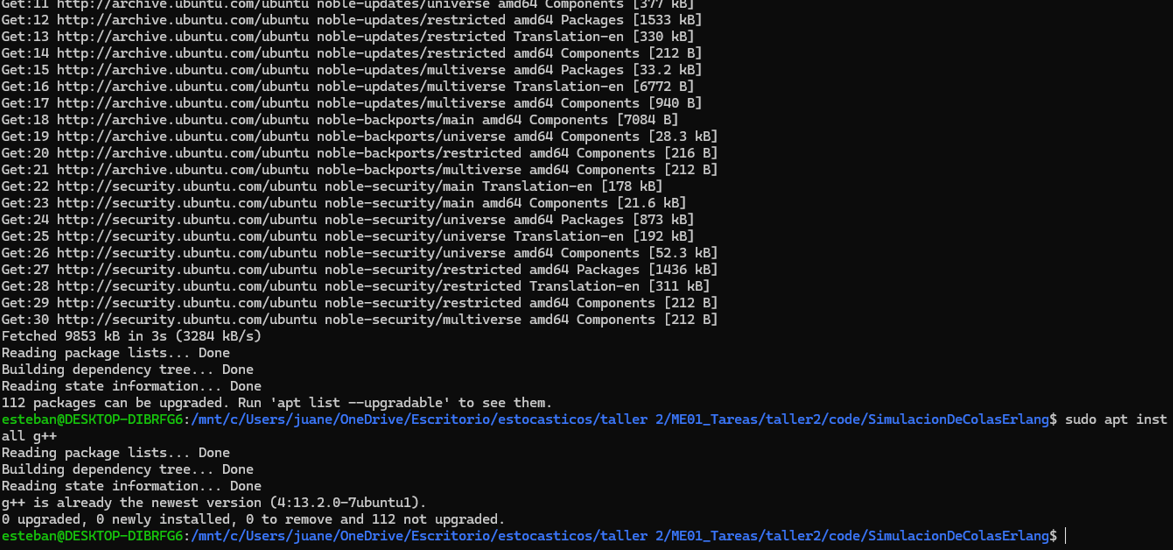
\includegraphics[width=0.8\textwidth]{images/manualUsuarioErlangBC_1.png}
    \caption{Proceso de instalación de g++}
    \label{fig:instalacion}
\end{figure}

Verificación de la instalación:
\begin{verbatim}
g++ --version
\end{verbatim}

\begin{figure}[H]
    \centering
    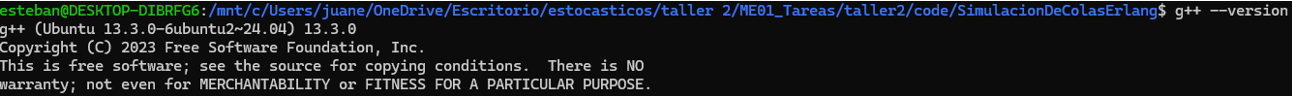
\includegraphics[width=0.8\textwidth]{images/manualUsuarioErlangBC_2.png}
    \caption{Verificación de la versión de g++}
    \label{fig:version}
\end{figure}

\subsubsection{Instalación de Ubuntu en WSL (Opcional)}
En caso de que se esté trabajando en windows hay varias alternativas para compilar y ejecutar el codigo c++. Acá presentamos una por medio de Ubuntu en WSL. Para instalarlo siga los siguientes pasos:

\begin{enumerate}
    \item Verificar/Activar característica WSL
    
    Ir al panel de control y seleccionar ``desistalar un programa`` en la sección de programas

    \begin{figure}[H]
    \centering
    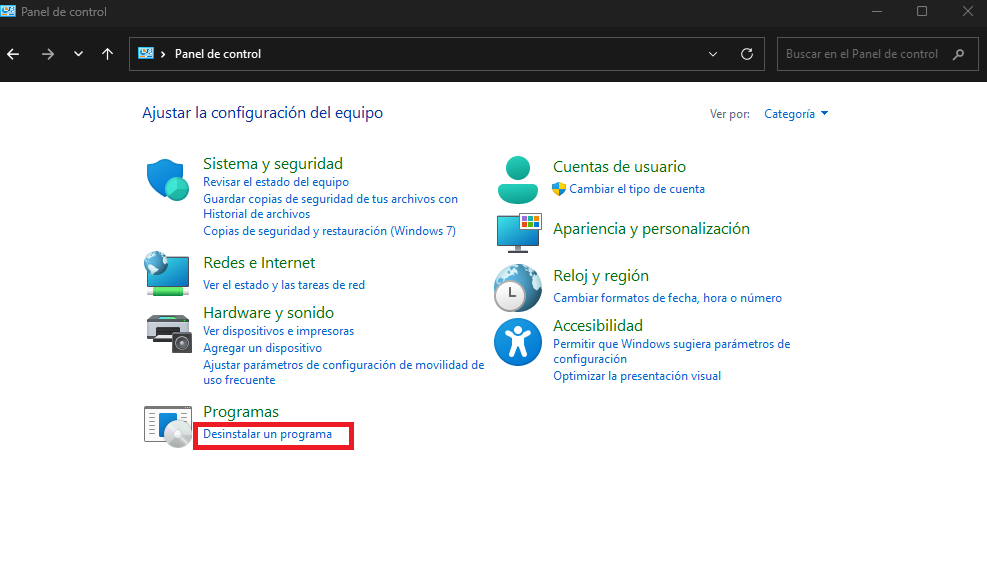
\includegraphics[width=0.8\textwidth]{images/manualUsuarioErlangBC_6.png}
    \caption{Panel de Control}
    \label{fig:version}
\end{figure}

A continuación a la izquierda encontrará ``Activar o desactivar las características de Windows`` al oprimirlo le abrirá una ventana donde debe verificar que la casilla ``Subsistema de Windows para Linux`` este seleccionada, en caso de no estarlo seleccionela

\begin{figure}[H]
    \centering
    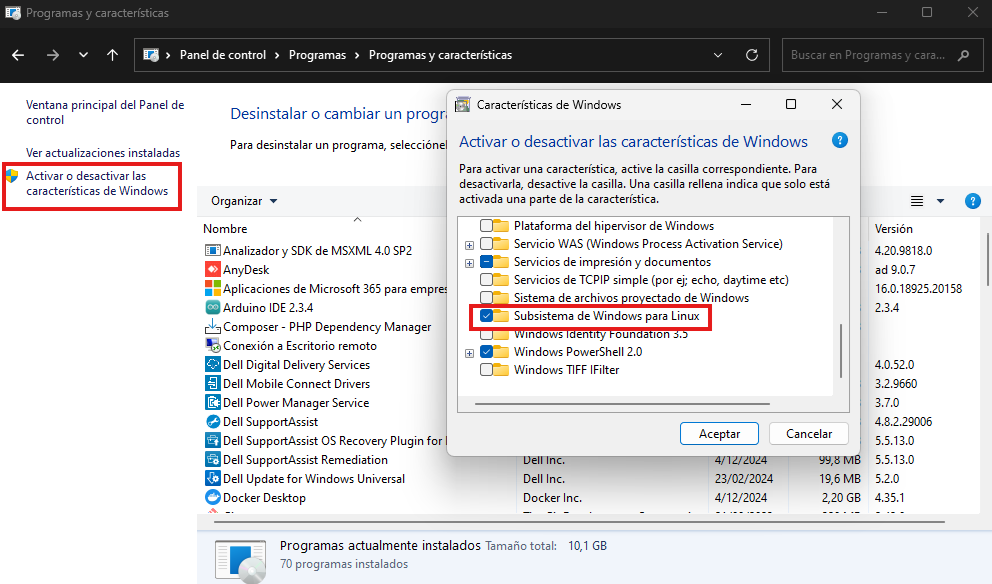
\includegraphics[width=0.8\textwidth]{images/manualUsuarioErlangBC_7.png}
    \caption{Características de Windows}
    \label{fig:version}
\end{figure}

    \item Instalación
    
    Vaya a Microsoft Store y busque Ubuntu, oprima la primera opción y despues ``Obtener``, acá se instalará. Pueden salir cuadros de dialogo para pedir permisos, oprima aceptar. Una vez finalizada la descarga abra el programa.

    \begin{figure}[H]
    \centering
    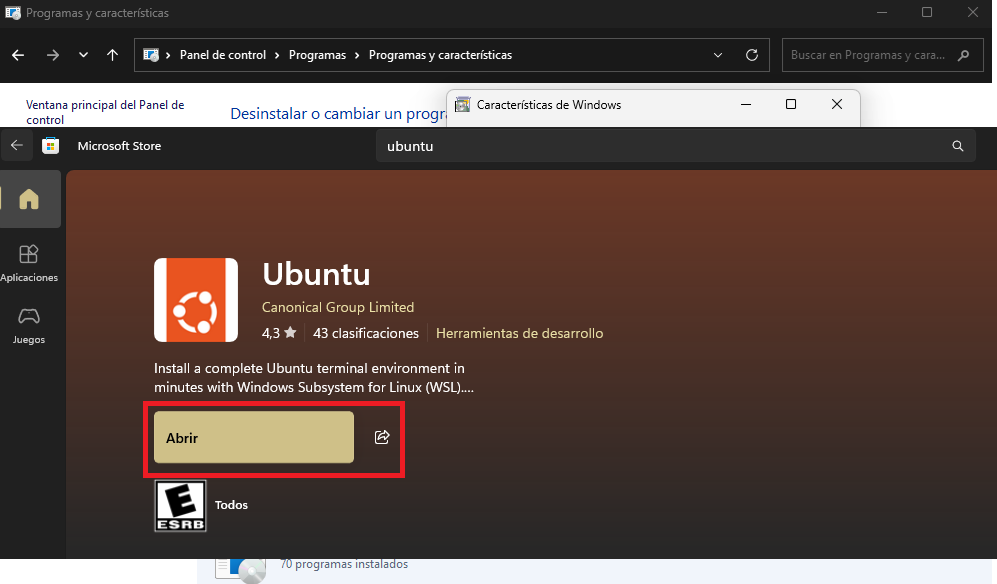
\includegraphics[width=0.8\textwidth]{images/manualUsuarioErlangBC_8.png}
    \caption{Microsoft Store}
    \label{fig:version}
\end{figure}

Finalmente siga los pasos para configurar el usuario y ejecute cualquier comando para verificar su correcto funcionamiento (Puede ussar el comando ls).

\begin{figure}[H]
    \centering
    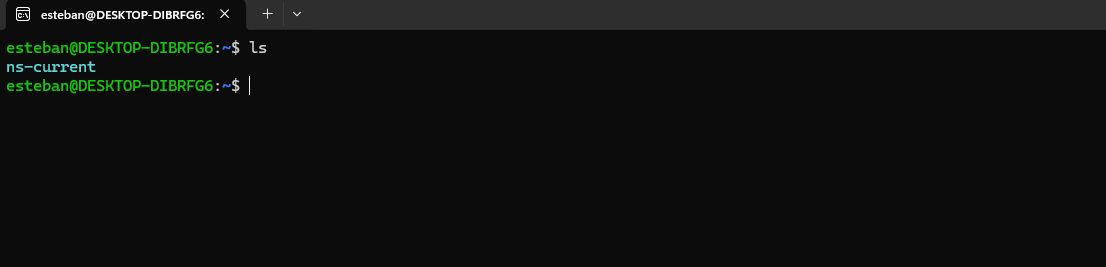
\includegraphics[width=0.8\textwidth]{images/manualUsuarioErlangBC_9.png}
    \caption{Instalación exitosa de Ubuntu en WSL}
    \label{fig:version}
\end{figure}

\end{enumerate}

\subsubsection{Configuración de parámetros}
Los parámetros de simulación se configuran en el archivo 
\texttt{param.txt} ubicado en \texttt{taller2/code/}
\texttt{SimulacionDeColasErlang}. Los parámetros son:

\begin{itemize}
    \item \texttt{media\_entre\_llegadas}: Tiempo medio entre llegadas (float)
    \item \texttt{media\_atencion}: Tiempo medio de atención (float)
    \item \texttt{num\_esperas\_requerido}: Número de esperas a simular (integer)
    \item \texttt{modo}: Tipo de modelo Erlang (0 para B, 1 para C)
    \item \texttt{num\_servidores}: Cantidad de servidores (integer)
\end{itemize}

\begin{figure}[H]
    \centering
    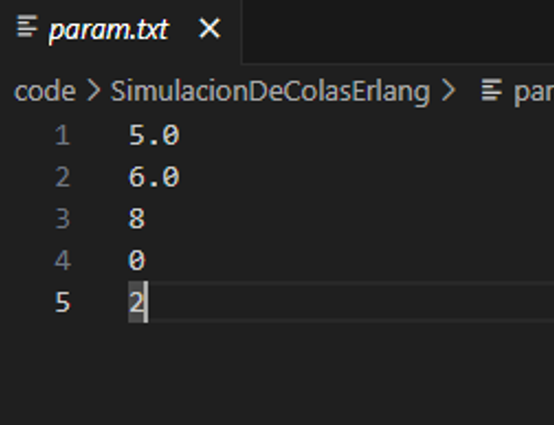
\includegraphics[width=0.8\textwidth]{images/manualUsuarioErlangBC_3.png}
    \caption{Ejemplo de archivo de parámetros}
    \label{fig:parametros}
\end{figure}

\subsubsection{Compilación y ejecución}
Proceso para compilar y ejecutar:

1. Compilación del programa:
\begin{verbatim}
g++ Sistema\ de\ Colas.cpp -o SistemaDeColas
\end{verbatim}

2. Ejecución del simulador:
\begin{verbatim}
./SistemaDeColas
\end{verbatim}

\begin{figure}[H]
    \centering
    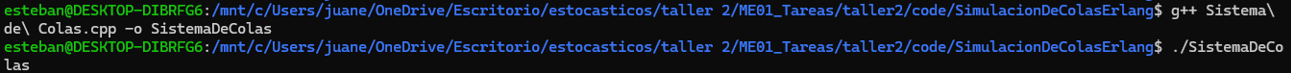
\includegraphics[width=0.8\textwidth]{images/manualUsuarioErlangBC_4.png}
    \caption{Proceso de compilación y ejecución}
    \label{fig:compilacion}
\end{figure}

\subsubsection{Resultados}
El programa genera un archivo \texttt{result.txt} con:

\begin{figure}[H]
    \centering
    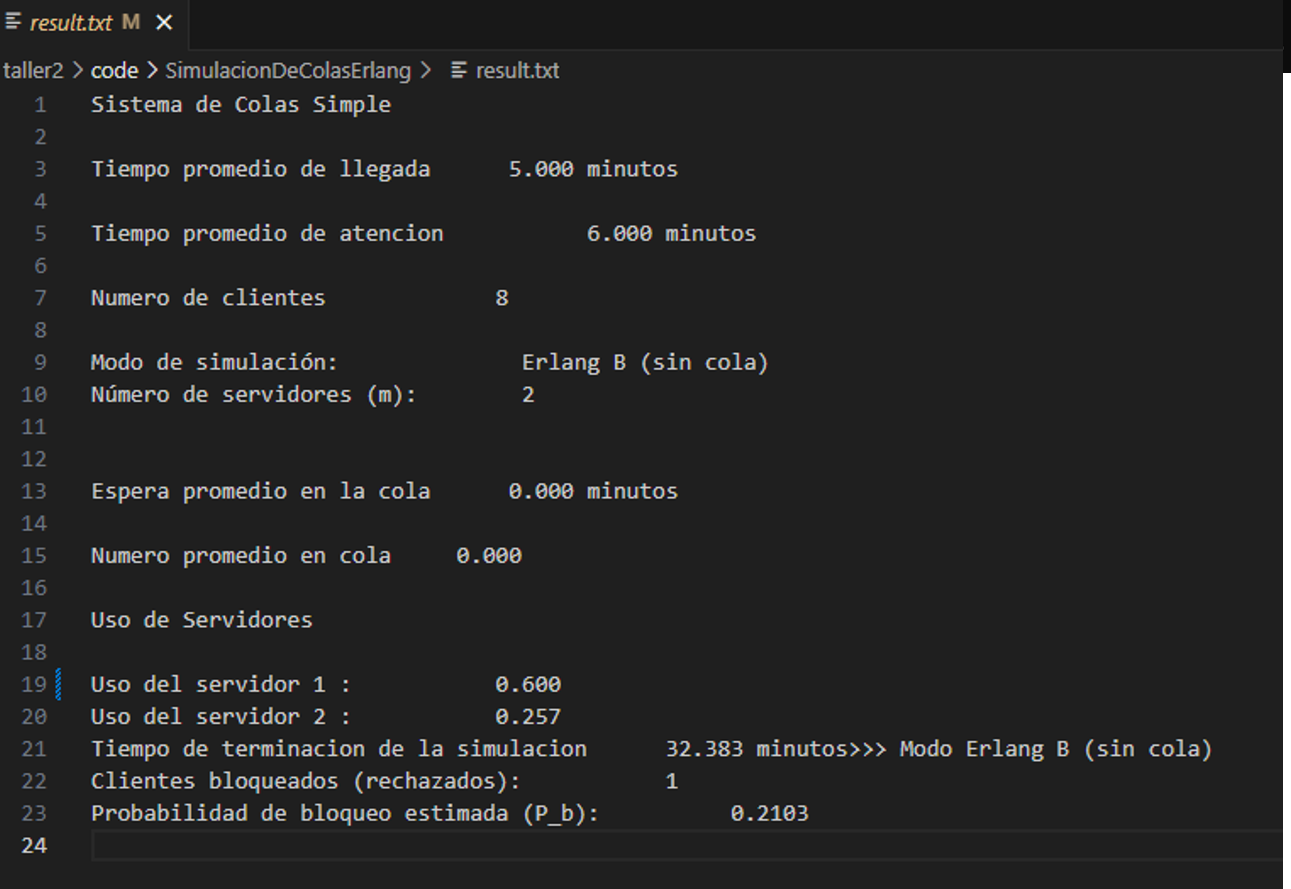
\includegraphics[width=0.8\textwidth]{images/manualUsuarioErlangBC_5.png}
    \caption{Ejemplo de archivo de resultados}
    \label{fig:resultados}
\end{figure}

La estructura del archivo incluye primero los parámetros de entrada, como los tiempos promedio de llegada y atención, el número de clientes simulados y la configuración de servidores. Luego, muestra los resultados principales, como la probabilidad de bloqueo, el uso de cada servidor y métricas de desempeño (tiempos de espera y ocupación). Finalmente, indica el tiempo total de simulación y el número de clientes rechazados. Este formato permite analizar rápidamente el comportamiento del sistema y la eficiencia de los recursos.

%---------------------------------------------------------------------------------
% Manual técnico ------------------------------------------------------------------
%---------------------------------------------------------------------------------

\section{Manual Técnico}

\subsection{Geo/Geo/m}\label{subsec:geogeo_m}

Simulador de un sistema de colas $(Geom/Geom/m):(FIFO/N/+ \infty)$ implementado en C++. El programa modela un sistema de colas con llegadas y servicios geométricos, múltiples servidores (m), capacidad finita (N) y disciplina FIFO.

\subsubsection{Prerequisitos}

\begin{itemize}
    \item Compilador C++ compatible con C++11 o superior
    \item Bibliotecas estándar: \texttt{stdio.h}, \texttt{stdlib.h}, \texttt{math.h}, \texttt{time.h}, \texttt{vector}
    \item Generador de números aleatorios proporcionado en \texttt{lcgrand.cpp}
    \item Sistema operativo: Windows/Linux/macOS
\end{itemize}

\subsubsection{Estructura del código}

El programa sigue una estructura modular con las siguientes componentes principales:

\begin{itemize}
    \item \textbf{Variables globales}:
    \begin{itemize}
        \item Parámetros del sistema (N, m, p, s, num\_slots)
        \item Estado del sistema (estado\_actual, servidores\_ocupados, cola\_length)
        \item Estadísticas (tiempo\_en\_estado[], clientes\_perdidos, clientes\_llegados)
    \end{itemize}
    
    \item \textbf{Funciones principales}:
    \begin{itemize}
        \item \texttt{main()}: Coordina el flujo del programa
        \item \texttt{inicializar()}: Prepara el sistema para la simulación
        \item \texttt{simular\_slot()}: Avanza la simulación un paso de tiempo
        \item \texttt{calcular\_estadisticas()}: Calcula métricas de desempeño
    \end{itemize}
    
    \item \textbf{Funciones auxiliares}:
    \begin{itemize}
        \item Generación aleatoria: \texttt{generar\_bernoulli()}, \texttt{generar\_binomial()}
        \item Cálculos matemáticos: \texttt{factorial()}, \texttt{potencia()}, \texttt{comb()}
        \item Modelo teórico: \texttt{geom\_geom\_m\_N\_p\_calc()}, \texttt{a\_func()}
    \end{itemize}
\end{itemize}

\subsubsection{Parámetros de la simulación}

Los parámetros se leen del archivo \texttt{paramGeo.txt} con el formato:

\begin{verbatim}
N m p s num_slots
\end{verbatim}

Donde:
\begin{itemize}
    \item \textbf{N}: Capacidad máxima del sistema (clientes)
    \item \textbf{m}: Número de servidores
    \item \textbf{p}: Probabilidad de llegada en un slot
    \item \textbf{s}: Probabilidad de finalización de servicio en un slot
    \item \textbf{num\_slots}: Duración de la simulación (slots)
\end{itemize}

\subsubsection{Salidas de la simulación}

El programa genera tres archivos de salida:

\begin{itemize}
    \item \texttt{estadisticas.txt}: Distribución de probabilidad del número de clientes en el sistema y probabilidad de bloqueo
    \item \texttt{comparacion\_teorica.txt}: Comparación entre resultados simulados y teóricos
    \item \texttt{resumen\_resultados.txt}: Métricas agregadas (utilización, promedio de clientes, throughput)
\end{itemize}

\subsubsection{Funciones principales}

\paragraph{\texttt{main()}}
\begin{itemize}
    \item Lee parámetros de \texttt{paramGeo.txt}
    \item Inicializa el sistema
    \item Ejecuta el bucle principal de simulación
    \item Coordina el cálculo y reporte de resultados
\end{itemize}

\paragraph{\texttt{simular\_slot()}}
\begin{itemize}
    \item Genera llegadas usando distribución Bernoulli(p)
    \item Genera salidas usando distribución Binomial(servidores\_ocupados, s)
    \item Actualiza el estado del sistema
    \item Registra estadísticas
\end{itemize}

\paragraph{\texttt{geom\_geom\_m\_N\_p\_calc()}}
Implementa el algoritmo para calcular las probabilidades de estado estacionario teóricas según el modelo Geom/Geom/m/N, basado en:
\begin{itemize}
    \item Thomas G. Robertazzi \textit{Computer Networks and Systems: Queueing Theory and Performance Evaluation Third Edition}
    \item 6.4 The Geom/Geom/m/N Queing system
\end{itemize}

\paragraph{\texttt{a\_func()}}
Función auxiliar que calcula $a_{i,j} \ 's$

\subsubsection{Compilación y ejecución}

Para compilar y ejecutar el simulador:

\begin{verbatim}
g++ sistemaGeoGeo.cpp -o sistemaGeoGeo 
./sistemaGeoGeo
\end{verbatim}

\subsubsection{Extensión del código}

Para modificar o extender el código:
\begin{itemize}
    \item Para cambiar el generador de números aleatorios, modificar \texttt{lcgrand.cpp}
    \item Para añadir nuevas métricas, extender \texttt{calcular\_estadisticas()}
    \item Para cambiar el modelo de llegadas/servicios, modificar \texttt{simular\_slot()}
\end{itemize}




%---------------------------------------------------------------------------------
% Exprimentación ------------------------------------------------------------------
%---------------------------------------------------------------------------------


\section{Experimentación}\label{sec:exp}

\subsection{Erlang B, probabilidad de bloqueo}\label{subsec:erlang_b_prob_bloq}

Para validar el simulador, se realizó un experimento con los siguientes parámetros:

\begin{itemize}
    \item Media entre llegadas ($\lambda$): 5 minutos
    \item Media de atención ($\mu$): 6 minutos
    \item Número de clientes a simular: 100
    \item Modo: 0 (Erlang B, sin cola)
    \item Número de servidores ($m$): 2
\end{itemize}

\textbf{Cálculo teórico:}

La fórmula de Erlang B para la probabilidad de bloqueo $p_m$ es:
\begin{equation*}
p_m = \frac{\frac{1}{m!}\left(\frac{\lambda}{\mu}\right)^m}{1 + \sum_{n=1}^{m} \frac{1}{n!}\left(\frac{\lambda}{\mu}\right)^n}
\end{equation*}
donde:
\begin{itemize}
    \item $\lambda$ es la tasa de llegadas
    \item $\mu$ es la tasa de servicio
    \item $m$ es el número de servidores
\end{itemize}

Para este caso:
\begin{align*}
    \lambda &= 1/5 \text{ clientes/minuto} \\
    \mu &= 1/6 \text{ clientes/minuto} \\
    A &= \frac{1/5}{1/6} = 1.2 \\
    m &= 2
\end{align*}

\begin{align*}
p_m &= \frac{\frac{1}{2!}\left(\frac{1/5}{1/6}\right)^2}{1 + \frac{1}{1!}\left(\frac{1/5}{1/6}\right)^1 + \frac{1}{2!}\left(\frac{1/5}{1/6}\right)^2} \\
    &= \frac{\frac{1}{2}\cdot(1.2)^2}{1 + 1.2 + \frac{1}{2}\cdot(1.2)^2} \\
    &= \frac{0.72}{2.92} \approx 0.2466
\end{align*}

\textbf{Resultados simulados:}

\begin{verbatim}
Sistema de Colas Simple

Tiempo promedio de llegada      5.000 minutos
Tiempo promedio de atencion           6.000 minutos
Numero de clientes           100
Modo de simulación:              Erlang B (sin cola)
Número de servidores (m):        2
Espera promedio en la cola      0.000 minutos
Numero promedio en cola     0.000
Uso de Servidores
Uso del servidor 1 :           0.021
Uso del servidor 2 :           0.544
Tiempo de terminacion de la simulacion     982.220 minutos>>> Modo Erlang B (sin cola)
Clientes bloqueados (rechazados):           105
Probabilidad de bloqueo estimada (P_b):          0.5426
\end{verbatim}

\textbf{Análisis:}

El valor simulado de la probabilidad de bloqueo ($P_b = 0.5426$) es considerablemente mayor que el valor teórico ($\approx 0.2466$). Esto es esperable cuando el número de clientes simulados es bajo (100), ya que la variabilidad estadística es mucho mayor y los resultados pueden alejarse del valor teórico. Para obtener una mejor aproximación al valor teórico, se recomienda aumentar el número de clientes simulados (por ejemplo, a 10,000 o más).

\subsection{Erlang C, probabilidad de espera}\label{subsec:erlang_c_prob_espe}

Para validar el simulador bajo el modelo Erlang C (con cola), se realizó un experimento con los siguientes parámetros:

\begin{itemize}
    \item Media entre llegadas ($\lambda$): 5 minutos
    \item Media de atención ($\mu$): 6 minutos
    \item Número de clientes a simular: 100
    \item Modo: 1 (Erlang C, con cola)
    \item Número de servidores ($m$): 2
\end{itemize}

\textbf{Cálculo teórico:}

La fórmula de Erlang C para la probabilidad de que un cliente tenga que esperar (haya cola) es:
\begin{equation*}
p(\text{cola}) = \frac{\frac{1}{m!}\left(\frac{\lambda}{\mu}\right)^m \left( \frac{1}{1-\rho} \right)}{1 + \sum_{n=1}^{m-1} \frac{1}{n!}\left(\frac{\lambda}{\mu}\right)^n + \frac{1}{m!}\left(\frac{\lambda}{\mu}\right)^m \left( \frac{1}{1-\rho} \right)}
\end{equation*}
donde:
\begin{itemize}
    \item $\lambda$ es la tasa de llegadas
    \item $\mu$ es la tasa de servicio
    \item $m$ es el número de servidores
    \item $\rho = \frac{\lambda}{m\mu}$ es la utilización del sistema
\end{itemize}

Para este caso:
\begin{align*}
    \lambda &= 1/5 \text{ clientes/minuto} \\
    \mu &= 1/6 \text{ clientes/minuto} \\
    m &= 2 \\
    \rho &= \frac{1/5}{2 \times 1/6} = \frac{1/5}{1/3} = 0.6
\end{align*}

\begin{align*}
p(\text{cola}) &= \frac{\frac{1}{2!}\left(1.2\right)^2 \left( \frac{1}{1-0.6} \right)}{1 + \frac{1}{1!}(1.2)^1 + \frac{1}{2!}(1.2)^2 \left( \frac{1}{1-0.6} \right)} \\
    &= \frac{0.72 \times 2.5}{1 + 1.2 + 0.72 \times 2.5} \\
    &= \frac{1.8}{4.0} = 0.45
\end{align*}

\textbf{Resultados simulados:}

\begin{verbatim}
Sistema de Colas Simple

Tiempo promedio de llegada      5.000 minutos
Tiempo promedio de atencion           6.000 minutos
Numero de clientes           100
Modo de simulación:              Erlang C (con cola)
Número de servidores (m):        2

Espera promedio en la cola      7.972 minutos
Numero promedio en cola     1.330
Uso de Servidores
Uso del servidor 1 :           0.026
Uso del servidor 2 :           0.782
Tiempo de terminacion de la simulacion     599.268 minutos>>> Modo Erlang C (con cola)
Clientes que debieron esperar:              70
Probabilidad de espera estimada (P_w):           0.7761
\end{verbatim}

\textbf{Análisis:}

Dado que el número de clientes simulados es bajo (100), es esperable que la probabilidad de espera simulada difiera del valor teórico ($0.45$) debido a la alta variabilidad estadística inherente a muestras pequeñas. Esto puede provocar que el valor simulado sea mayor o menor que el teórico, y que la dispersión entre ejecuciones sea significativa. Para obtener una mejor aproximación al valor teórico, se recomienda aumentar el número de clientes simulados (por ejemplo, a 10,000 o más), lo que reduce la variabilidad y permite que la simulación converja hacia el valor esperado por la teoría de colas. Si la diferencia entre el valor simulado y el teórico persiste incluso con muestras grandes, se recomienda revisar la correcta interpretación de los parámetros y la implementación del simulador.

\subsection{Erlang C, probabilidad de espera con más servidores}

Para analizar el efecto de aumentar el número de servidores en la probabilidad de espera, se realizó un experimento bajo el modelo Erlang C (con cola) con los siguientes parámetros:

\begin{itemize}
    \item Media entre llegadas ($\lambda$): 5 minutos
    \item Media de atención ($\mu$): 6 minutos
    \item Número de clientes a simular: 100
    \item Modo: 1 (Erlang C, con cola)
    \item Número de servidores ($m$): 5
\end{itemize}

\textbf{Cálculo teórico:}

La fórmula de Erlang C para la probabilidad de que un cliente tenga que esperar (haya cola) es:
\begin{equation*}
p(\text{cola}) = \frac{\frac{1}{m!}\left(\frac{\lambda}{\mu}\right)^m \left( \frac{1}{1-\rho} \right)}{1 + \sum_{n=1}^{m-1} \frac{1}{n!}\left(\frac{\lambda}{\mu}\right)^n + \frac{1}{m!}\left(\frac{\lambda}{\mu}\right)^m \left( \frac{1}{1-\rho} \right)}
\end{equation*}
donde:
\begin{itemize}
    \item $\lambda$ es la tasa de llegadas
    \item $\mu$ es la tasa de servicio
    \item $m$ es el número de servidores
    \item $\rho = \frac{\lambda}{m\mu}$ es la utilización del sistema
\end{itemize}

Para este caso:
\begin{align*}
    \lambda &= 1/5 \text{ clientes/minuto} \\
    \mu &= 1/6 \text{ clientes/minuto} \\
    m &= 5 \\
    \rho &= \frac{1/5}{5 \times 1/6} = \frac{1/5}{5/6} = 0.24 \\
    \frac{\lambda}{\mu} &= 1.2
\end{align*}

\begin{align*}
p(\text{cola}) &= \frac{\frac{1}{5!}(1.2)^5 \left( \frac{1}{1-0.24} \right)}{1 + \sum_{n=1}^{4} \frac{1}{n!}(1.2)^n + \frac{1}{5!}(1.2)^5 \left( \frac{1}{1-0.24} \right)} = 0.0082
\end{align*}

\textbf{Resultados simulados:}

\begin{verbatim}
Sistema de Colas Simple

Tiempo promedio de llegada      5.000 minutos

Tiempo promedio de atencion           6.000 minutos

Numero de clientes           100

Modo de simulación:              Erlang C (con cola)
Número de servidores (m):        5

Espera promedio en la cola      7.158 minutos

Numero promedio en cola     1.249

Uso de Servidores

Uso del servidor 1 :           0.026
Uso del servidor 2 :           0.012
Uso del servidor 3 :           0.091
Uso del servidor 4 :           0.032
Uso del servidor 5 :           0.704
Tiempo de terminacion de la simulacion     573.145 minutos>>> Modo Erlang C (con cola)
Clientes que debieron esperar:              60
Probabilidad de espera estimada (P_w):           0.6944
\end{verbatim}

\textbf{Análisis comparativo:}

Al comparar este resultado con el experimento anterior con 2 servidores (donde la probabilidad de espera simulada fue $P_w = 0.7761$), se observa que, aunque la probabilidad de espera disminuye al aumentar el número de servidores, en este caso sigue siendo relativamente alta ($P_w = 0.6944$). Esto puede deberse a la alta variabilidad estadística por el bajo número de clientes simulados (100) o a la configuración de los parámetros de llegada y servicio. 

Teóricamente, al aumentar los servidores, el sistema debería ser capaz de atender a más clientes sin que tengan que esperar, y la probabilidad de espera debería disminuir considerablemente. Para observar esta reducción de manera más clara y obtener una mejor aproximación al valor teórico, se recomienda aumentar el número de clientes simulados (por ejemplo, a 10,000 o más). Si la probabilidad de espera sigue siendo alta incluso con muestras grandes, es importante revisar la correcta interpretación de los parámetros y la implementación del simulador para descartar errores o malentendidos en la lógica del modelo.

\section{Referencias}
\renewcommand{\refname}{}
\begin{thebibliography}{9}

\bibitem{ref} \label{ref:modSim} A. M. Law, *Simulation Modeling and Analysis*, 5th ed. 
New York, NY, USA: McGraw-Hill Education, Jan. 2014, ISBN 978-0-07-340132-4. 

\bibitem{ref} \label{ref:matSim} J. E. Ortiz T., "Modelos Matemáticos \& Simulación,"
 en *Apuntes de clase de la asignatura Modelos Estocásticos y Simulación en 
 Computación y Comunicaciones*, Departamento de Ingeniería de Sistemas e Industrial, 
 Universidad Nacional de Colombia, 2025. [En línea]. Disponible en: 
 \url{https://drive.google.com/file/d/1c886yU4SFk9A97DGWr8JHiF3nd2au1Ns/view?usp=sharing}

 \bibitem{ref} \label{ref:cimColas} J. E. UOrtiz, "Simulador del modelo de colas M/M/1," 
 código fuente en C++ (archivo .rar), basado en la sección 
 1.4.4 de Averill M. Law, *Simulation Modeling and Analysis*, 
 th ed., McGraw-Hill, 2014. [En línea]. Disponible en: 
 \url{https://drive.google.com/file/d/1-Mo9hqPwOegwTpx0KP2tbD9sLTNSXefd/view?usp=sharing}



\end{thebibliography}

\end{document}